% day3_seg1_navproblem/coordconv.tex
\begin{frame}
\frametitle{Coordinate Frames}
 \begin{itemize}
 \item Inertial
 \item Earth Fixed
 \item Local Level
 \item Body
\end{itemize}
\end{frame}
\begin{frame}
\frametitle{Coordinate Frames}
 \begin{itemize}
  \item Technically speaking, all frames are earth-centered
  \begin{itemize}
    \item Common origen needed for linear transformations (such as rotations)
    \item Can compensate by using a translation
  \end{itemize}
  \item Practically speaking, we think of the Body frame as centered in the body of the vehicle (usually at center of gravity).
  \item Local Level is thought to be located at surface of earth directly beneath the vehicle.
\end{itemize}
\end{frame}
\begin{frame}
\frametitle{Inertial Reference Frames}
 \begin{itemize}
 \item Non-Rotating
 \item Non-Accelerating
 \item Fixed or moving uniformly with respect to another inertial
 frame (fixed stars)
\end{itemize}
\end{frame}

\begin{frame}
\frametitle{Inertial Reference Frames}
 \begin{itemize}
 \item Nav problem "easy" in inertial frames
 \item Integrate gyro rates once to get attitude (rotational motion independent of lateral motion)
 \item Rotate accelerometer outputs to inertial frame using attitude matrix, then integrate to get inertial
 velocity; integrate velocity to get position.
 \item Would still have to contend with instrument imperfections.
\end{itemize}
\end{frame}

\begin{frame}
\frametitle{Inertial Reference Frame Integrations}
\begin{equation}\label{inertacceleq}
\ddot{r}(t)=\specforce+\text{other external forces}
\end{equation}
\begin{equation}\label{inertveleq}
v(T)=\dot{r}(T)=v(0)+\int_{0}^{T}\specforce dt + \int_{0}^{T}(\text{other
external forces})dt
\end{equation}
\begin{equation}\label{inertposeq}
  r(T)=r(0)+\int_{0}^{T}v(t)dt
\end{equation}
\end{frame}

\begin{frame}
\frametitle{Earth Fixed = ECEF = Earth Centered Earth Fixed}
 \begin{itemize}
 \item Rotating frame, i.e., non-inertial
 \item Cartesian ($X,Y,Z$ in meters)
 \item Spherical (latitude $\lat$, longitude $\lon$, altitude $\alt$)
 \begin{itemize}
 \item geodetic
 \end{itemize}
\end{itemize}
\end{frame}


\begin{frame}
\frametitle{Local Level}
 \begin{itemize}
 \item Tangent to earth's surface but translated to center of
 earth.
 \item Vertical $Z$-axis is normal to earth's surface
 \item $X,Y$-axes are level
 \item Several kinds: $Y$ north-slaved, wander (0 transport rate) or free azimuth
 \item $Y$ makes wander angle $\alpha$ with respect to true north (ENU=East, North, Up).
\end{itemize}
\end{frame}

\begin{frame}
\frametitle{Earth Centered, Earth Fixed:  ECEF}
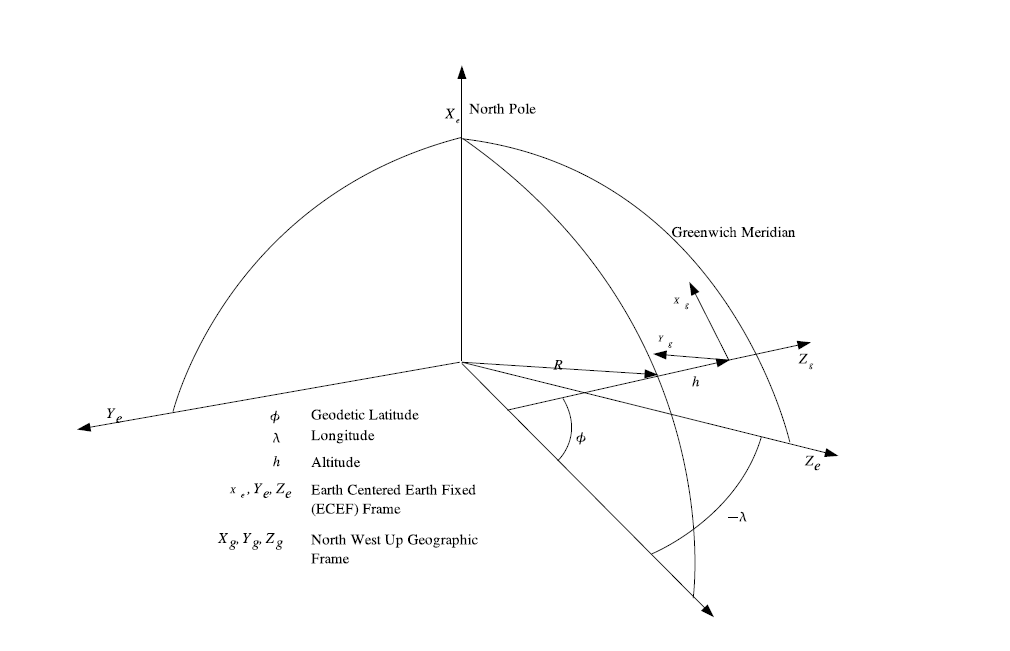
\includegraphics[width=\textwidth]{graphics/ecef.png}
\vfill
\end{frame}


\begin{frame}
\frametitle{Body Frame}
 \begin{itemize}
 \item Attached to vehicle
 \item For aircraft:
   \begin{itemize}
    \item $X$ out the nose
    \item $Y$ out the right wing
    \item $Z$ down
   \end{itemize}
\end{itemize}
\end{frame}

\begin{frame}
\frametitle{Body Frame (cont)}
 \begin{itemize}
 \item For space vehicles RIC:
   \begin{itemize}
    \item $R$ downward on radius to center of earth
    \item $I$ in-track, in direction of motion
    \item $C$ cross-track, perpendicular to motion
   \end{itemize}
 \item Also sometimes referred as RAC, where 'A' stands for 'along-track'
\end{itemize}
\end{frame}

\begin{frame}
\frametitle{Coordinate Frame Conversion}
 \begin{itemize}
 \item All frames earth-centered, differing only by
 rotation
 \item Rotation represented by direction cosine matrix (DCM) or set of four quaternions
 \begin{itemize}
	\item Expresses angles made by basis vectors of one frame with those of another
 \end{itemize}
 \item $\dcm{A}{B}$ = DCM transformation from frame A to frame B
\end{itemize}
\end{frame}

\begin{frame}
\frametitle{Coordinate Frame Conversion}
\begin{itemize}
  \item "Direction Cosine" comes from dot product:
\[\ip{x}{y}=x\cdot y=\norm{x}\norm{y}\cos\theta_{xy}\]
where $\theta_{xy}$ is the angle between the two vectors $x$ and $y$.
  \item If $x$ and $y$ are unit vectors, then $\norm{x}=\norm{y}=1$ and we have:
\[\ip{x}{y}=x\cdot y=\cos\theta_{xy}\]
\end{itemize} 
\end{frame}

\begin{frame}
\frametitle{Coordinate Frame Conversion}
\begin{itemize}
  \item If $U=\set{u_1,u_2,u_3}$ and $V=\set{v_1,v_2,v_3}$ are two sets of orthonormal basis vectors, then the DCM relating one frame to the other is given by:
\begin{align*}
\dcm{U}{V}&=
\begin{bmatrix}
\ip{u_1}{v_1} & \ip{u_1}{v_2} & \ip{u_1}{v_3}\\
\ip{u_2}{v_1} & \ip{u_2}{v_1} & \ip{u_2}{v_3}\\
\ip{u_3}{v_1} & \ip{u_3}{v_2} & \ip{u_3}{v_3}\\
\end{bmatrix}\\
&=
\begin{bmatrix}
\cos\theta_{11} & \cos\theta_{12} & \cos\theta_{13}\\
\cos\theta_{21} & \cos\theta_{22} & \cos\theta_{23}\\
\cos\theta_{31} & \cos\theta_{32} & \cos\theta_{33}\\
\end{bmatrix}
\end{align*}
\end{itemize} 
\end{frame}

\begin{frame}
\frametitle{Coordinate Frame Conversion}
\begin{itemize}
  \item If $V=\set{v_1,v_2,v_3}$ is considered to be the reference frame and its units vectors are the standard basis so that 
\[
v_1=\begin{bmatrix}
	1\\
	0\\
	0\\
	\end{bmatrix},
v_2=\begin{bmatrix}
	0\\
	1\\
	0\\
	\end{bmatrix},
v_3=\begin{bmatrix}
	0\\
	0\\
	1\\
	\end{bmatrix},
\]
then the DCM simplifies to just the coordinates of $u_1,u_2,u_3$ vectors with respect to $V$:
\begin{align*}
\dcm{U}{V}&=
\begin{bmatrix}
u_{11}& u_{12} & u_{13}\\
u_{21} & u_{22} & u_{23}\\
u_{31} & u_{32} & u_{33}\\
\end{bmatrix}
\end{align*}
\end{itemize} 
\end{frame}


\begin{frame}
\frametitle{Coordinate Frame Conversion}
 \begin{itemize}
 \item DCMs are (real) orthogonal matrices $\Rightarrow \left[\dcm{A}{B} \right]^{-1}=\left[\dcm{A}{B} \right]\trans=\dcm{B}{A}$
 \item Third row (or column) is vector cross product of other two\\
 $\Rightarrow$ only six independent parameters
 \item DCMs satisfy:   $\dcm{B}{A}\dcm{C}{B}=\dcm{C}{A}$
\end{itemize}
\end{frame}

\begin{frame}
\frametitle{Coordinate Frame Conversion}
 \begin{itemize}
 \item Orthogonal matrices preserve lengths of vectors: $\norm{Rx}=\norm{x}$
 \item Orthogonal matrices also preserve angles between vectors:  $\ip{Rx}{Ry}=\ip{R\trans Rx}{y}=\ip{Ix}{y}=\ip{x}{y}$
 \item Intuitively obvious in the case of rotations
\end{itemize}
\end{frame}

\begin{frame}
\frametitle{DCMs and Euler Rotation}
 \begin{itemize}
 \item Euler showed that three simultaneous rotations about three orthogonal axes can be
viewed as a single rotation about a single axis
 \item The single angle $\theta$ of rotation for a DCM can be determined from the eigenvalues of the DCM, which are:
\[
\set{1, \exp(i\theta), \exp(-i\theta)}
\]
\item The determinant of a DCM is therefore always 1.   Why? (Hint: How do you compute the determinant from the eigenvalues?)
\end{itemize}
\end{frame}

\begin{frame}
\frametitle{Euler Rotation}
\begin{figure}[h]
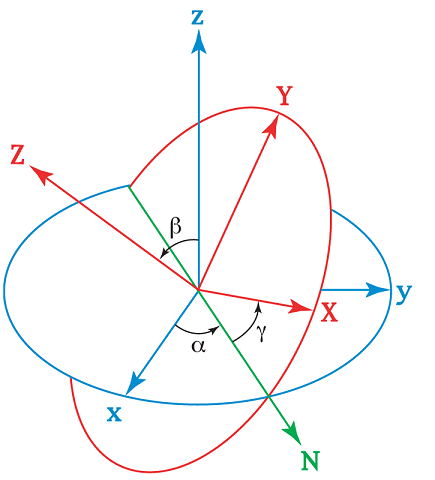
\includegraphics[width=0.5\textwidth]{graphics/euler.png}
\end{figure}
\end{frame}


\begin{frame}
\frametitle{DCMs and Euler Rotation}
 \begin{itemize}
 \item The axis of rotation for the single Euler rotation can be found from DCM as follows:
\begin{align*}
\dcm{U}{V}&=
\begin{bmatrix}
u_{11}& u_{12} & u_{13}\\
u_{21} & u_{22} & u_{23}\\
u_{31} & u_{32} & u_{33}\\
\end{bmatrix}
\end{align*}
then the axis of rotation $r = [r_1,r_2,r_3]\trans$ is given by
\begin{align*}
r_1 &= u_{12}u_{23} - (u_{22}-1)u_{13}\\
r_2 &= u_{21}u_{13} - (u_{11}-1)u_{23}\\
r_3 &= (u_{11}-1)(u_{22}-1) - u_{12}u_{21}\\
\end{align*}
\end{itemize}
\end{frame}

\begin{frame}
\frametitle{DCMs and Quaternions}
 \begin{itemize}
 \item If $C$ is a direction cosine matrix with elements $c_{ij}$, then the following four quantities define a quaternion of the rotation:
\begin{align*}
q_1 &= \dfrac{1}{4q_4}(c_{23}-c_{32})\\
q_2 &= \dfrac{1}{4q_4}(c_{13}-c_{31})\\
q_3 &= \dfrac{1}{4q_4}(c_{21}-c_{12})\\
q_4 &= \pm \dfrac{1}{2}\sqrt{1+c_{11}+c_{22}+c_{33}}\\
\end{align*}
\end{itemize}
\end{frame}

\begin{frame}
\frametitle{DCMs and Quaternions}
 \begin{itemize}
 \item It's even simpler to obtain quaternions from Euler rotation angle $\theta$ and axis given by a unit vector $u$:
\[q_i=u_i\sin(\theta/2), \text{ for } i=1,2,3\]
and
\[q_4=\cos(\theta/2)\]
\end{itemize}
\end{frame}


\begin{frame}
\frametitle{Coordinate Frame Conversion: Most important DCMs for terrestrial navigation}
 \begin{itemize}
 \item Body to Local Level: $\dcm{B}{L}$
 \begin{itemize}
 \item sometimes called Body to Nav and notated $\dcm{B}{N}$
 \item yields attitude info (Euler angles for roll, pitch, yaw)
 \end{itemize}
 \item Local Level to Earth: $\dcm{L}{E}$
 \begin{itemize}
 \item yields position info and also used to transform earth rate to
 local level
 \end{itemize}
\end{itemize}
\end{frame}
\begin{frame}
\frametitle{Coordinate Frame Conversion: Most important DCMs}
\begin{itemize}
  \item Visualize $\dcm{L}{E}$'s determination of position as follows:
	\begin{itemize}
		\item As vehicle moves, local level frame changes its orienation with respect to earth's center in order to maintain local level with respect to earth's surface
		\item If you think of local level frame as attached to earth's surface, you get distracted by the displacement of the frame
		\item If you move local level frame to center of earth, the displacement disappears and all that remains are the rotations
	\end{itemize} 
\end{itemize} 
\end{frame}

\begin{frame}
\begin{figure}
\centering
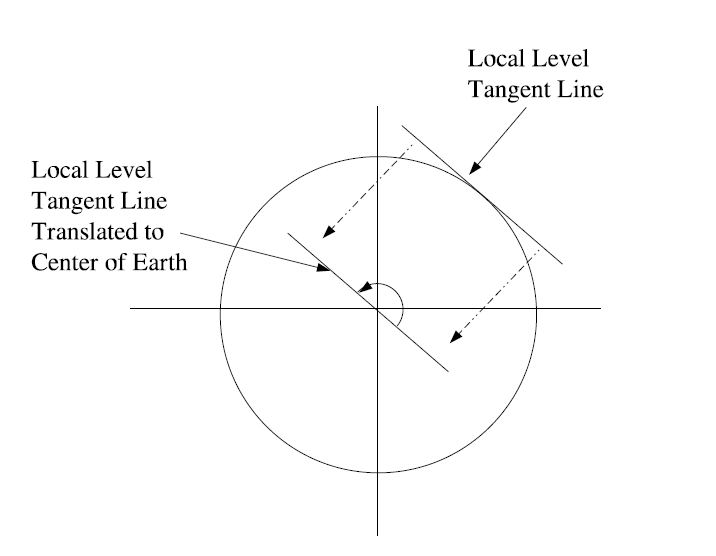
\includegraphics[width=\textwidth]{graphics/local_level.png}
\caption{Local Level to Earth Transformation}
\end{figure}
\end{frame}